\subsection{Einführung}
Das Toolkit \emph{Basemap} ist ein Pythonmodul zur Bearbeitung von Karten.
Es bietet viele verschiedene Arten Karten in 2D darzustellen (siehe Projektionen \ref{Projektionen} )
Es ermöglicht einem auch das Plotten auf den Karten. Hierbei kann man, dann auch Längen- und Breitengrad als Positionsangabe nutzen. Das \emph{Basemap} Toolkit wandelt die Koordinaten dann mit der \emph{PROJ4} Library in die entsprechenden 2D Koordinaten um. Beim Plotten greift das Modul auf Funktionen des Moduls \emph{pyplot} und \emph{matplotlib} zurück. Der große Vorteil beim benutzen des \textsf{Basemap} Moduls ist, dass es die geografischen Koordinaten sehr einfach umrechnet. Was einem die Definition der Projektionsalgorithmen abnimmt. Des weiteren hat dieses Modul sehr präzise Umrissdaten, was es ermöglicht die Länder sehr genau darzustellen. Es bietet auch gröbere Umrissdaten, wenn man nicht so viel Rechenzeit hat. Mit diesem Modul ist es äußerst einfach, meteorologische Karten zu erstellen. Da es viele Funktionen bereitstellt mit denen man die Daten direkt darstellen kann. Es gibt Funktionen, um Windmarken oder Vektoren zu zeichnen. Andere Funktionen zeichnen Isobaren oder Strömungsgraphen oder farbig gefüllte Isobaren, diese können einfach zum Darstellen von Niederschlag verwendet werden. Diese Funktionen müssen einfach nur mit den Daten aufgerufen werden, diese Daten können auch als Felder vorliegen. Da das Modul das umrechnen der Koordinaten sehr einfach macht, können die Daten meistens einfach aus den Eingabedateien in die Felder gelesen werden, dies ist in \textsf{Python} sehr leicht.
 In diesem Kapitel werde ich die Funktionen von \textsf{Basemap} an einem Beispiel vorstellen. Bei diesem Beispiel werde ich die äquidistante Zylinderprojektion benutzen. Diese Projektion verwende ich, da sie die einfachste Projektion ist. Ich werde dabei darauf achten das die Beispiele auch mit anderen Projektionen funktionieren könnten.\\
 Hier ein Beispiel zum umrechnen von Koordinaten
\lstinputlisting{/Users/student/seminar/bsp/bspconvert.py}
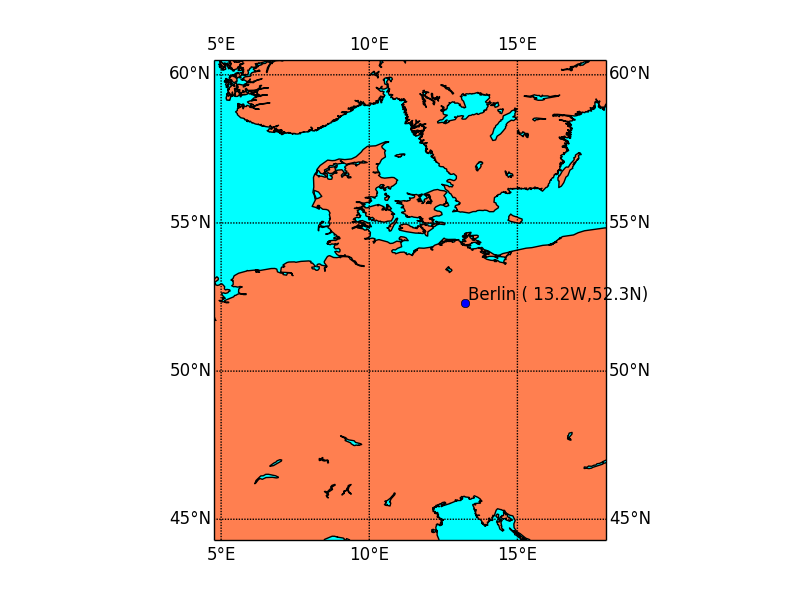
\includegraphics[scale=0.4]{/Users/student/seminar/bsp/bspconvert} 